% Options for packages loaded elsewhere
\PassOptionsToPackage{unicode}{hyperref}
\PassOptionsToPackage{hyphens}{url}
%
\documentclass[
]{article}
\usepackage{amsmath,amssymb}
\usepackage{lmodern}
\usepackage{iftex}
\ifPDFTeX
  \usepackage[T1]{fontenc}
  \usepackage[utf8]{inputenc}
  \usepackage{textcomp} % provide euro and other symbols
\else % if luatex or xetex
  \usepackage{unicode-math}
  \defaultfontfeatures{Scale=MatchLowercase}
  \defaultfontfeatures[\rmfamily]{Ligatures=TeX,Scale=1}
\fi
% Use upquote if available, for straight quotes in verbatim environments
\IfFileExists{upquote.sty}{\usepackage{upquote}}{}
\IfFileExists{microtype.sty}{% use microtype if available
  \usepackage[]{microtype}
  \UseMicrotypeSet[protrusion]{basicmath} % disable protrusion for tt fonts
}{}
\makeatletter
\@ifundefined{KOMAClassName}{% if non-KOMA class
  \IfFileExists{parskip.sty}{%
    \usepackage{parskip}
  }{% else
    \setlength{\parindent}{0pt}
    \setlength{\parskip}{6pt plus 2pt minus 1pt}}
}{% if KOMA class
  \KOMAoptions{parskip=half}}
\makeatother
\usepackage{xcolor}
\usepackage[margin=1in]{geometry}
\usepackage{color}
\usepackage{fancyvrb}
\newcommand{\VerbBar}{|}
\newcommand{\VERB}{\Verb[commandchars=\\\{\}]}
\DefineVerbatimEnvironment{Highlighting}{Verbatim}{commandchars=\\\{\}}
% Add ',fontsize=\small' for more characters per line
\usepackage{framed}
\definecolor{shadecolor}{RGB}{248,248,248}
\newenvironment{Shaded}{\begin{snugshade}}{\end{snugshade}}
\newcommand{\AlertTok}[1]{\textcolor[rgb]{0.94,0.16,0.16}{#1}}
\newcommand{\AnnotationTok}[1]{\textcolor[rgb]{0.56,0.35,0.01}{\textbf{\textit{#1}}}}
\newcommand{\AttributeTok}[1]{\textcolor[rgb]{0.77,0.63,0.00}{#1}}
\newcommand{\BaseNTok}[1]{\textcolor[rgb]{0.00,0.00,0.81}{#1}}
\newcommand{\BuiltInTok}[1]{#1}
\newcommand{\CharTok}[1]{\textcolor[rgb]{0.31,0.60,0.02}{#1}}
\newcommand{\CommentTok}[1]{\textcolor[rgb]{0.56,0.35,0.01}{\textit{#1}}}
\newcommand{\CommentVarTok}[1]{\textcolor[rgb]{0.56,0.35,0.01}{\textbf{\textit{#1}}}}
\newcommand{\ConstantTok}[1]{\textcolor[rgb]{0.00,0.00,0.00}{#1}}
\newcommand{\ControlFlowTok}[1]{\textcolor[rgb]{0.13,0.29,0.53}{\textbf{#1}}}
\newcommand{\DataTypeTok}[1]{\textcolor[rgb]{0.13,0.29,0.53}{#1}}
\newcommand{\DecValTok}[1]{\textcolor[rgb]{0.00,0.00,0.81}{#1}}
\newcommand{\DocumentationTok}[1]{\textcolor[rgb]{0.56,0.35,0.01}{\textbf{\textit{#1}}}}
\newcommand{\ErrorTok}[1]{\textcolor[rgb]{0.64,0.00,0.00}{\textbf{#1}}}
\newcommand{\ExtensionTok}[1]{#1}
\newcommand{\FloatTok}[1]{\textcolor[rgb]{0.00,0.00,0.81}{#1}}
\newcommand{\FunctionTok}[1]{\textcolor[rgb]{0.00,0.00,0.00}{#1}}
\newcommand{\ImportTok}[1]{#1}
\newcommand{\InformationTok}[1]{\textcolor[rgb]{0.56,0.35,0.01}{\textbf{\textit{#1}}}}
\newcommand{\KeywordTok}[1]{\textcolor[rgb]{0.13,0.29,0.53}{\textbf{#1}}}
\newcommand{\NormalTok}[1]{#1}
\newcommand{\OperatorTok}[1]{\textcolor[rgb]{0.81,0.36,0.00}{\textbf{#1}}}
\newcommand{\OtherTok}[1]{\textcolor[rgb]{0.56,0.35,0.01}{#1}}
\newcommand{\PreprocessorTok}[1]{\textcolor[rgb]{0.56,0.35,0.01}{\textit{#1}}}
\newcommand{\RegionMarkerTok}[1]{#1}
\newcommand{\SpecialCharTok}[1]{\textcolor[rgb]{0.00,0.00,0.00}{#1}}
\newcommand{\SpecialStringTok}[1]{\textcolor[rgb]{0.31,0.60,0.02}{#1}}
\newcommand{\StringTok}[1]{\textcolor[rgb]{0.31,0.60,0.02}{#1}}
\newcommand{\VariableTok}[1]{\textcolor[rgb]{0.00,0.00,0.00}{#1}}
\newcommand{\VerbatimStringTok}[1]{\textcolor[rgb]{0.31,0.60,0.02}{#1}}
\newcommand{\WarningTok}[1]{\textcolor[rgb]{0.56,0.35,0.01}{\textbf{\textit{#1}}}}
\usepackage{graphicx}
\makeatletter
\def\maxwidth{\ifdim\Gin@nat@width>\linewidth\linewidth\else\Gin@nat@width\fi}
\def\maxheight{\ifdim\Gin@nat@height>\textheight\textheight\else\Gin@nat@height\fi}
\makeatother
% Scale images if necessary, so that they will not overflow the page
% margins by default, and it is still possible to overwrite the defaults
% using explicit options in \includegraphics[width, height, ...]{}
\setkeys{Gin}{width=\maxwidth,height=\maxheight,keepaspectratio}
% Set default figure placement to htbp
\makeatletter
\def\fps@figure{htbp}
\makeatother
\setlength{\emergencystretch}{3em} % prevent overfull lines
\providecommand{\tightlist}{%
  \setlength{\itemsep}{0pt}\setlength{\parskip}{0pt}}
\setcounter{secnumdepth}{-\maxdimen} % remove section numbering
\usepackage{booktabs}
\usepackage{longtable}
\usepackage{array}
\usepackage{multirow}
\usepackage{wrapfig}
\usepackage{float}
\usepackage{colortbl}
\usepackage{pdflscape}
\usepackage{tabu}
\usepackage{threeparttable}
\usepackage{threeparttablex}
\usepackage[normalem]{ulem}
\usepackage{makecell}
\usepackage{xcolor}
\ifLuaTeX
  \usepackage{selnolig}  % disable illegal ligatures
\fi
\IfFileExists{bookmark.sty}{\usepackage{bookmark}}{\usepackage{hyperref}}
\IfFileExists{xurl.sty}{\usepackage{xurl}}{} % add URL line breaks if available
\urlstyle{same} % disable monospaced font for URLs
\hypersetup{
  pdftitle={Assignment2},
  pdfauthor={Alejandro Pachón, Santiago Meza, Alexander Morgan},
  hidelinks,
  pdfcreator={LaTeX via pandoc}}

\title{Assignment2}
\author{Alejandro Pachón, Santiago Meza, Alexander Morgan}
\date{2023-04-21}

\begin{document}
\maketitle

\hypertarget{github}{%
\subsection{GitHub}\label{github}}

Puedes visitar nuestro repositorio en internet, para más información :
\href{https://github.com/Alejandro29-tech/Assignment2}{\textbf{Nuestro
Repositorio}}

\hypertarget{data-acquisition}{%
\subsection{1.1 Data acquisition}\label{data-acquisition}}

\hypertarget{sensor-ultrasonido-hc-sr04}{%
\subsection{Sensor ultrasonido
HC-SR04}\label{sensor-ultrasonido-hc-sr04}}

El sensor de ultrasonido HC-SR04 es un sensor popular utilizado para
medir distancias. en caunto asu funcionamiento, El HC-SR04 emite una
serie de pulsos de ultrasonido y mide el tiempo que tarda en recibir el
eco de estos pulsos. Utiliza esta información para calcular la distancia
desde el sensor hasta el objeto.El rango de medición del HC-SR04 es de 2
cm a 4 metros. en cuanto a su precicion es +/- de aproximadamente 3 mm.
su angulo de apertura es de 15° respecto al centro del emisor y trabaja
bajo una frecuencia de 40KHz, tambien utiliza como interfaaz de
comunicacion el sistema de PWM para enviar o recibir señales. para mas
infomacion se puede consultar el
\href{http://www.datasheetcafe.com/hc-sr04-pdf-22772/}{\textbf{Datasheet}}

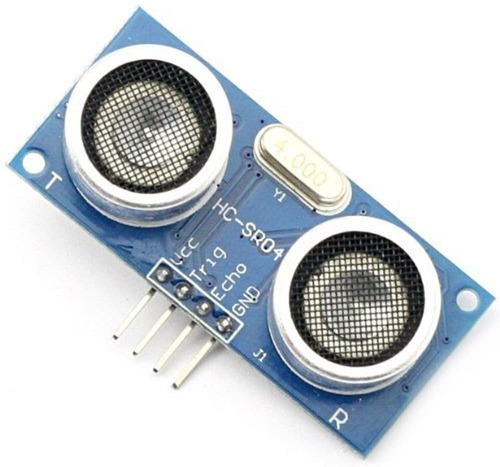
\includegraphics{images/hc-01.PNG})\{width=``280''\}

\hypertarget{sensor-infrarrojo-sharp-2y0a21}{%
\subsection{Sensor infrarrojo Sharp
2Y0A21}\label{sensor-infrarrojo-sharp-2y0a21}}

El Sharp 2Y0A21 emite un haz de luz infrarroja y mide la cantidad de luz
reflejada por un objeto para calcular la distancia mediante un
procesador integrado encargado de realizar el cálculo, El rango de
medición es de 10 cm a 80 cm. su precision es de +/- aproximadamente 1
cm. funciona con una frecuancia de 38KHz y su angulo de deteccion es de
25°, en el aspecto de comunicacion no cuenta con una propia simplemente
devuelve una tensión analógica proporcional a la distancia medida. para
mas infomacion se puede consultar el
\href{https://global.sharp/products/device/lineup/data/pdf/datasheet/gp2y0a21yk_e.pdf}{\textbf{Datasheet}}

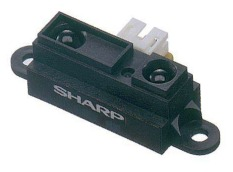
\includegraphics[width=2.91667in,height=\textheight]{images/2y.PNG}

\hypertarget{data-acquisition-1}{%
\subsection{2.1 Data acquisition}\label{data-acquisition-1}}

the following sensors are used to perform this data acquisition and data
projection project.

\begin{Shaded}
\begin{Highlighting}[]
\FunctionTok{library}\NormalTok{(dplyr)}
\FunctionTok{library}\NormalTok{(tidyverse)}
\end{Highlighting}
\end{Shaded}

\begin{verbatim}
## Warning: package 'tibble' was built under R version 4.2.3
\end{verbatim}

\begin{Shaded}
\begin{Highlighting}[]
\FunctionTok{library}\NormalTok{(readxl)}
\FunctionTok{library}\NormalTok{(knitr) }
\FunctionTok{library}\NormalTok{(kableExtra)}
\end{Highlighting}
\end{Shaded}

\begin{verbatim}
## Warning: package 'kableExtra' was built under R version 4.2.3
\end{verbatim}

\begin{Shaded}
\begin{Highlighting}[]
\CommentTok{\# Leer el archivo Excel}
\NormalTok{datos }\OtherTok{\textless{}{-}} \FunctionTok{read\_excel}\NormalTok{(}\StringTok{"\textasciitilde{}/UNIVERSIDAD/8vo Semestre/Area electronica (electiva)/Assignment2/R/1.1.xlsx"}\NormalTok{)}
\NormalTok{tabla\_adq}\OtherTok{\textless{}{-}}\FunctionTok{kable}\NormalTok{(datos)}
\NormalTok{tabla\_adq }\OtherTok{\textless{}{-}}\NormalTok{ tabla\_adq }\SpecialCharTok{\%\textgreater{}\%}
  \FunctionTok{kable\_styling}\NormalTok{(}\AttributeTok{full\_width =} \ConstantTok{FALSE}\NormalTok{)}
\NormalTok{tabla\_adq}
\end{Highlighting}
\end{Shaded}

\begin{table}
\centering
\begin{tabular}{r|r|r|r|r}
\hline
Sensor1 & Sensor1\_cm & cm & Sensor2 & Sensor2\_cm\\
\hline
1994 & 20 & 21.25 & 21.25 & 514\\
\hline
1201 & 20 & 21.30 & 21.30 & 513\\
\hline
1264 & 21 & 21.64 & 21.64 & 506\\
\hline
1388 & 23 & 23.44 & 23.44 & 472\\
\hline
1477 & 25 & 24.70 & 24.70 & 451\\
\hline
1605 & 27 & 26.09 & 26.09 & 430\\
\hline
1740 & 29 & 27.95 & 27.95 & 405\\
\hline
1838 & 31 & 29.11 & 29.11 & 391\\
\hline
1897 & 32 & 30.26 & 30.26 & 378\\
\hline
1953 & 33 & 31.50 & 31.50 & 365\\
\hline
2020 & 34 & 33.28 & 33.28 & 348\\
\hline
2110 & 36 & 34.89 & 34.89 & 334\\
\hline
2158 & 37 & 35.87 & 35.87 & 326\\
\hline
2254 & 38 & 37.32 & 37.32 & 315\\
\hline
2307 & 39 & 38.88 & 38.88 & 304\\
\hline
2376 & 40 & 40.56 & 40.56 & 293\\
\hline
2460 & 42 & 42.73 & 42.73 & 280\\
\hline
2550 & 43 & 43.99 & 43.99 & 273\\
\hline
2588 & 44 & 44.94 & 44.94 & 268\\
\hline
2642 & 45 & 46.33 & 46.33 & 261\\
\hline
2745 & 47 & 47.58 & 47.58 & 255\\
\hline
2775 & 47 & 48.90 & 48.90 & 249\\
\hline
2861 & 49 & 50.06 & 50.06 & 244\\
\hline
2930 & 50 & 52.27 & 52.27 & 235\\
\hline
2992 & 51 & 53.58 & 53.58 & 230\\
\hline
3080 & 52 & 55.52 & 55.52 & 223\\
\hline
3130 & 53 & 55.23 & 55.23 & 224\\
\hline
3184 & 54 & 57.59 & 57.59 & 216\\
\hline
3256 & 55 & 59.49 & 59.49 & 210\\
\hline
3323 & 57 & 62.21 & 62.21 & 202\\
\hline
3339 & 57 & 62.21 & 62.21 & 202\\
\hline
3401 & 58 & 63.65 & 63.65 & 198\\
\hline
3430 & 58 & 63.65 & 63.65 & 198\\
\hline
3470 & 58 & 71.03 & 71.03 & 180\\
\hline
3558 & 59 & 67.98 & 67.98 & 187\\
\hline
3596 & 61 & 67.98 & 67.98 & 187\\
\hline
3610 & 62 & 69.25 & 69.25 & 184\\
\hline
3672 & 63 & 72.89 & 72.89 & 176\\
\hline
3749 & 64 & 71.03 & 71.03 & 180\\
\hline
3786 & 65 & 72.89 & 72.89 & 176\\
\hline
3860 & 66 & 73.85 & 73.85 & 174\\
\hline
3864 & 66 & 75.34 & 75.34 & 171\\
\hline
3873 & 66 & 74.34 & 74.34 & 173\\
\hline
3875 & 66 & 76.89 & 76.89 & 168\\
\hline
3954 & 67 & 76.37 & 76.37 & 169\\
\hline
3948 & 67 & 76.89 & 76.89 & 168\\
\hline
3951 & 68 & 79.05 & 79.05 & 164\\
\hline
4004 & 68 & 77.96 & 77.96 & 164\\
\hline
4029 & 69 & 79.96 & 79.96 & 166\\
\hline
4083 & 70 & 79.05 & 79.05 & 168\\
\hline
4092 & 70 & 79.05 & 79.05 & 160\\
\hline
4159 & 71 & 81.33 & 81.33 & 163\\
\hline
\end{tabular}
\end{table}

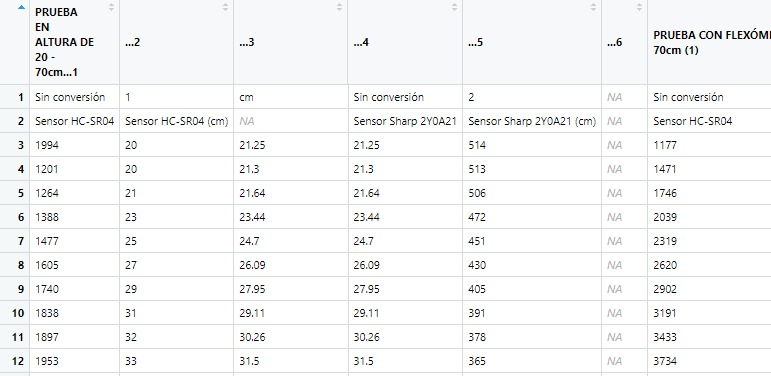
\includegraphics{images/adq1.PNG}

\hypertarget{modelo-lineal-para-hc-sr04-sensor1}{%
\subsection{Modelo lineal para HC-SR04
(Sensor1)}\label{modelo-lineal-para-hc-sr04-sensor1}}

El sensor de ultrasonido HC-SR04 es una herramienta utilizada para medir
distancias en proyectos electrónicos. Sin embargo, es necesario crear un
modelo matemático que permita predecir las mediciones del sensor con
mayor precisión y eficacia. Una forma de lograr esto es mediante la
creación de un modelo lineal que relacione las mediciones del sensor con
las variables que afectan su desempeño. como se ve acontinuacion:

\begin{Shaded}
\begin{Highlighting}[]
\CommentTok{\# Modelo lineal para Sensor1}
\NormalTok{datos }\OtherTok{\textless{}{-}} \FunctionTok{read\_excel}\NormalTok{(}\StringTok{"\textasciitilde{}/UNIVERSIDAD/8vo Semestre/Area electronica (electiva)/Assignment2/R/1.1.xlsx"}\NormalTok{)}
\NormalTok{model\_lin\_Sensor\_1 }\OtherTok{\textless{}{-}} \FunctionTok{lm}\NormalTok{(Sensor1 }\SpecialCharTok{\textasciitilde{}}\NormalTok{ Sensor1\_cm, }\AttributeTok{data =}\NormalTok{ datos)}

\CommentTok{\# Modelo lineal regularizado para Sensor1}
\FunctionTok{library}\NormalTok{(glmnet)}
\end{Highlighting}
\end{Shaded}

\begin{verbatim}
## Warning: package 'glmnet' was built under R version 4.2.3
\end{verbatim}

\begin{Shaded}
\begin{Highlighting}[]
\NormalTok{X}\OtherTok{\textless{}{-}}\FunctionTok{as.matrix}\NormalTok{(datos[,}\FunctionTok{c}\NormalTok{(}\StringTok{"Sensor1\_cm"}\NormalTok{,}\StringTok{"cm"}\NormalTok{)])}
\NormalTok{y}\OtherTok{\textless{}{-}}\FunctionTok{as.matrix}\NormalTok{(datos[,}\FunctionTok{c}\NormalTok{(}\StringTok{"Sensor1"}\NormalTok{)])}
\NormalTok{model\_reg\_Sensor\_1 }\OtherTok{\textless{}{-}} \FunctionTok{glmnet}\NormalTok{(X, y, }\AttributeTok{alpha =} \DecValTok{1}\NormalTok{)}

\CommentTok{\# Modelo lineal para Sensor2}
\NormalTok{model\_lin\_Sensor2 }\OtherTok{\textless{}{-}} \FunctionTok{lm}\NormalTok{(Sensor2 }\SpecialCharTok{\textasciitilde{}}\NormalTok{ Sensor2\_cm, }\AttributeTok{data =}\NormalTok{ datos)}

\CommentTok{\# Modelo lineal regularizado para Sensor2}
\NormalTok{model\_reg\_Sensor2 }\OtherTok{\textless{}{-}} \FunctionTok{glmnet}\NormalTok{(}\FunctionTok{as.matrix}\NormalTok{(datos[,}\FunctionTok{c}\NormalTok{(}\StringTok{"Sensor2\_cm"}\NormalTok{,}\StringTok{"cm"}\NormalTok{)]), }\FunctionTok{as.matrix}\NormalTok{(datos[,}\FunctionTok{c}\NormalTok{(}\StringTok{"Sensor2"}\NormalTok{)]), }\AttributeTok{alpha =} \DecValTok{1}\NormalTok{)}
\end{Highlighting}
\end{Shaded}

\hypertarget{cargar-datos}{%
\subsection{2.1 Cargar datos}\label{cargar-datos}}

\begin{Shaded}
\begin{Highlighting}[]
\NormalTok{knitr}\SpecialCharTok{::}\NormalTok{opts\_chunk}\SpecialCharTok{$}\FunctionTok{set}\NormalTok{(}\AttributeTok{echo =} \ConstantTok{TRUE}\NormalTok{)}
\FunctionTok{library}\NormalTok{(tidyverse)}
\FunctionTok{library}\NormalTok{(glmnet)}
\FunctionTok{library}\NormalTok{(kableExtra)}

\CommentTok{\# Cambiar nombres de columnas}
\FunctionTok{colnames}\NormalTok{(datos) }\OtherTok{\textless{}{-}} \FunctionTok{c}\NormalTok{(}\StringTok{"Sensor1"}\NormalTok{, }\StringTok{"Sensor1\_cm"}\NormalTok{, }\StringTok{"cm"}\NormalTok{, }\StringTok{"Sensor2"}\NormalTok{, }\StringTok{"Sensor2\_cm"}\NormalTok{)}

\CommentTok{\# Visualizar tabla}
\FunctionTok{kable}\NormalTok{(datos[}\DecValTok{1}\SpecialCharTok{:}\DecValTok{10}\NormalTok{,], }\AttributeTok{caption =} \StringTok{"Primeros 10 datos del dataset"}\NormalTok{) }\SpecialCharTok{\%\textgreater{}\%} \FunctionTok{kable\_classic}\NormalTok{(}\StringTok{"striped"}\NormalTok{)}
\end{Highlighting}
\end{Shaded}

\begin{table}

\caption{\label{tab:unnamed-chunk-2}Primeros 10 datos del dataset}
\centering
\begin{tabular}[t]{r|r|r|r|r}
\hline
Sensor1 & Sensor1\_cm & cm & Sensor2 & Sensor2\_cm\\
\hline
1994 & 20 & 21.25 & 21.25 & 514\\
\hline
1201 & 20 & 21.30 & 21.30 & 513\\
\hline
1264 & 21 & 21.64 & 21.64 & 506\\
\hline
1388 & 23 & 23.44 & 23.44 & 472\\
\hline
1477 & 25 & 24.70 & 24.70 & 451\\
\hline
1605 & 27 & 26.09 & 26.09 & 430\\
\hline
1740 & 29 & 27.95 & 27.95 & 405\\
\hline
1838 & 31 & 29.11 & 29.11 & 391\\
\hline
1897 & 32 & 30.26 & 30.26 & 378\\
\hline
1953 & 33 & 31.50 & 31.50 & 365\\
\hline
\end{tabular}
\end{table}

\hypertarget{renombrar-las-columnas}{%
\subsection{Renombrar las columnas}\label{renombrar-las-columnas}}

\begin{Shaded}
\begin{Highlighting}[]
\FunctionTok{colnames}\NormalTok{(datos) }\OtherTok{\textless{}{-}} \FunctionTok{c}\NormalTok{(}\StringTok{"Sensor1"}\NormalTok{, }\StringTok{"Sensor1\_cm"}\NormalTok{, }\StringTok{"cm"}\NormalTok{, }\StringTok{"Sensor2"}\NormalTok{, }\StringTok{"Sensor2\_cm"}\NormalTok{)}
\end{Highlighting}
\end{Shaded}

\hypertarget{knn-para-el-sensor-1}{%
\subsection{KNN para el Sensor 1}\label{knn-para-el-sensor-1}}

Para el entrenamiento mediante el metodo e KNN para el sensor HC-SR04,
veremos cómo utilizar los datos de entrenamiento para determinar los k
vecinos más cercanos a una instancia desconocida y cómo clasificar o
predecir el valor de distancia basado en la mayoría de los valores de
los vecinos más cercanos.

\begin{Shaded}
\begin{Highlighting}[]
\FunctionTok{library}\NormalTok{(caret)}
\end{Highlighting}
\end{Shaded}

\begin{verbatim}
## Warning: package 'caret' was built under R version 4.2.3
\end{verbatim}

\begin{Shaded}
\begin{Highlighting}[]
\NormalTok{modelo\_sensor1 }\OtherTok{\textless{}{-}} \FunctionTok{train}\NormalTok{(Sensor1\_cm }\SpecialCharTok{\textasciitilde{}}\NormalTok{ cm, }\AttributeTok{data =}\NormalTok{ datos, }\AttributeTok{method =} \StringTok{"knn"}\NormalTok{)}
\end{Highlighting}
\end{Shaded}

\hypertarget{hacer-una-predicciuxf3n-para-un-nuevo-valor-de-sensor-1}{%
\subsection{Hacer una predicción para un nuevo valor de sensor
1}\label{hacer-una-predicciuxf3n-para-un-nuevo-valor-de-sensor-1}}

\begin{Shaded}
\begin{Highlighting}[]
\NormalTok{nuevo\_valor\_sensor1 }\OtherTok{\textless{}{-}} \DecValTok{20} \CommentTok{\# Por ejemplo}
\NormalTok{prediccion\_sensor1 }\OtherTok{\textless{}{-}} \FunctionTok{predict}\NormalTok{(modelo\_sensor1, }\AttributeTok{newdata =} \FunctionTok{data.frame}\NormalTok{(}\AttributeTok{cm =}\NormalTok{ nuevo\_valor\_sensor1))}
\end{Highlighting}
\end{Shaded}

\hypertarget{imprimir-la-predicciuxf3n-para-el-sensor-1}{%
\section{Imprimir la predicción para el Sensor
1}\label{imprimir-la-predicciuxf3n-para-el-sensor-1}}

\begin{Shaded}
\begin{Highlighting}[]
\FunctionTok{print}\NormalTok{(prediccion\_sensor1)}
\end{Highlighting}
\end{Shaded}

\begin{verbatim}
## [1] 21.8
\end{verbatim}

\hypertarget{entrenar-el-modelo-knn-para-el-sensor-2}{%
\subsection{Entrenar el modelo KNN para el Sensor
2}\label{entrenar-el-modelo-knn-para-el-sensor-2}}

\begin{Shaded}
\begin{Highlighting}[]
\NormalTok{modelo\_sensor2 }\OtherTok{\textless{}{-}} \FunctionTok{train}\NormalTok{(Sensor2\_cm }\SpecialCharTok{\textasciitilde{}}\NormalTok{ cm, }\AttributeTok{data =}\NormalTok{ datos, }\AttributeTok{method =} \StringTok{"knn"}\NormalTok{)}
\end{Highlighting}
\end{Shaded}

\hypertarget{hacer-una-predicciuxf3n-para-un-nuevo-valor-de-sensor-2}{%
\subsection{Hacer una predicción para un nuevo valor de sensor
2}\label{hacer-una-predicciuxf3n-para-un-nuevo-valor-de-sensor-2}}

\begin{Shaded}
\begin{Highlighting}[]
\NormalTok{nuevo\_valor\_sensor2 }\OtherTok{\textless{}{-}} \DecValTok{30} \CommentTok{\# Por ejemplo}
\NormalTok{prediccion\_sensor2 }\OtherTok{\textless{}{-}} \FunctionTok{predict}\NormalTok{(modelo\_sensor2, }\AttributeTok{newdata =} \FunctionTok{data.frame}\NormalTok{(}\AttributeTok{cm =}\NormalTok{ nuevo\_valor\_sensor2))}
\end{Highlighting}
\end{Shaded}

\hypertarget{imprimir-la-predicciuxf3n-para-el-sensor-2}{%
\section{Imprimir la predicción para el Sensor
2}\label{imprimir-la-predicciuxf3n-para-el-sensor-2}}

\begin{Shaded}
\begin{Highlighting}[]
\FunctionTok{print}\NormalTok{(prediccion\_sensor2)}
\end{Highlighting}
\end{Shaded}

\begin{verbatim}
## [1] 377.4
\end{verbatim}

\end{document}
